\documentclass[lettersize,journal]{IEEEtran}
\usepackage{amsmath,amsfonts}
\usepackage{algorithmic}
\usepackage{algorithm}
\usepackage{array}
\usepackage[caption=false,font=normalsize,labelfont=sf,textfont=sf]{subfig}
\usepackage{textcomp}
\usepackage{stfloats}
\usepackage{url}
\usepackage{verbatim}
\usepackage{graphicx}
\usepackage{cite}
\hyphenation{op-tical net-works semi-conduc-tor IEEE-Xplore}
% updated with editorial comments 8/9/2021

\begin{document}

\title{SC-407 and MC-226 Project}

\author{Om Gor (202101), Student2 Name (202101),\\ Student N Name (202101), Akshar Panchani (202101522)}

% The paper headers
\markboth{SC-407 Project: Group $18$}%
{Project Title}

% \IEEEpubid{0000--0000/00\$00.00~\copyright~2021 IEEE}
% Remember, if you use this you must call \IEEEpubidadjcol in the second
% column for its text to clear the IEEEpubid mark.

\maketitle

\begin{abstract}
Plastic pollution in the oceans poses a very significant threat to our marine ecosystems, biodiversity, human health, and countries economies. As this seems like a major concern to conserve and preserve our environment, we highlight the importance of marine life and address the efforts that should be made to reduce the plastic pollution in oceans.
\end{abstract}

\begin{IEEEkeywords}
Plastic Pollution, Marine Debris, Deep Learning, Autonomous Underwater Vehicles (AUVs), Object Detection, Conservation, Evaluation Metrics
\end{IEEEkeywords}

\section{Introduction}
\IEEEPARstart{P}{lastic} pollution has become a global challenge for many sectors, which include food safety, human health, marine life, and many more. Despite many efforts applied in this field, it still faces many problems, such as high cost, inaccurate assessment of plastic waste, labor work to solve such issues, and limitations to cover areas that are limited to rivers or lakes and do not cover large ocean bodies. Therefore, there is a need to have innovative solutions to address such issues globally.



\subsection{Problem Statement}
The major problem or the main cause includes the environmental harm to the water bodies in rivers, lakes, seas, and oceans. This is because currently more than 14 million metric tons of plastic are deposited in the ocean every year, causing the depletion of marine ecosystems. The current methods for monitoring marine plastic have high maintenance costs, higher building costs, and also require greater labor work. Moreover, the ocean is also polluted due to the rise of carbon dioxide in the environment, leading to the acidification of the water. So this brings in a solution to develop a machine learning model with computer vision to detect the plastic precisely and other marine debris throughout the entire water body.

\subsection{Relevant Works}
Many initiatives are being taken in this direction to protect our environment. The Government of France has recently implemented the anti-waste law to aim to curb single-use plastic that ends up in freshwater. \cite{France} It is noted that out of 14 million tons of plastic that end up in the ocean, 80\% of the marine debris is found on the surface of the water or deep-sea sediments. \cite{IUCN} For this, many studies have been conducted, such as the remote sensing technique, which can be used to conduct aerial surveys on water bodies to detect floating plastic. \cite{Invest} Research is made to analyze the underwater composition of plastic debris on the seafloor; this showcases the accumulation of plastic underwater. Many algorithms and the use of convolutional neural networks are used to quantify the issue. The SOTA for this is to deploy the autonomous underwater vehicles (AUVs), which are equipped with sensors and imaging systems to monitor marine plastic debris. They are capable of scanning large ocean beds. Many collaborative efforts are made by governments and NGOs to provide large datasets and databases for such technology that can detect plastic in the ocean. With the development of this ML model, the software aims to detect plastic in the ocean in order to collect those remains by the AUVs or by manual labor for small water bodies.


\subsection{Our Contributions}
In this study, we use deep learning and computer vision techniques to present a unique strategy to address the problems associated with monitoring marine plastic. Our method seeks to provide an accurate, dependable, and real-time system for measuring and identifying marine plastic waste across the whole water column. Our contribution consists of building on previous research and methods, diversifying datasets, introducing specific modifications, testing multiple object detection models, and assessing model performance with pertinent metrics.


\subsection{Organization}
The structure of this document is as follows. Section II gives a summary of our suggested methodology. The procedures and methodology used are covered in Section III. The experimental findings and assessment metrics are shown in Section IV. In Section V, the work is finally concluded and future directions for research are discussed.

\section{Proposed Approach}

This is the section with the meat of your idea. Here, you describe what you have done. 

It is good to have a general schematic and block diagrammatic representation of your idea. For example, you can include Fig.~\ref{fig_1}, which provides an overview of your proposed approach.

% \begin{figure}[!t]
% \centering
% \includegraphics[width=3.5in]{Fig2.pdf}
% \caption{Simulation results of the proposed approach.}
% \label{fig_1}
% \end{figure}

\subsection{An Analytical Derivation}

\subsubsection{Corollaries}

Organize the content of this section in different subsections, or even subsubsections, to make an impactful and well-organized presentation.

\section{Algorithms}
Algorithms should be numbered and include a short title. They are set off from the text with rules above and below the title and after the last line.

% \begin{algorithm}[H]
% \caption{Weighted Tanimoto ELM.}\label{alg:alg1}
% \begin{algorithmic}
% \STATE 
% \STATE {\textsc{TRAIN}}$(\mathbf{X} \mathbf{T})$
% \STATE \hspace{0.5cm}$ \textbf{select randomly } W \subset \mathbf{X}  $
% \STATE \hspace{0.5cm}$ N_\mathbf{t} \gets | \{ i : \mathbf{t}_i = \mathbf{t} \} | $ \textbf{ for } $ \mathbf{t}= -1,+1 $
% \STATE \hspace{0.5cm}$ B_i \gets \sqrt{ \textsc{max}(N_{-1},N_{+1}) / N_{\mathbf{t}_i} } $ \textbf{ for } $ i = 1,...,N $
% \STATE \hspace{0.5cm}$ \hat{\mathbf{H}} \gets  B \cdot (\mathbf{X}^T\textbf{W})/( \mathbb{1}\mathbf{X} + \mathbb{1}\textbf{W} - \mathbf{X}^T\textbf{W} ) $
% \STATE \hspace{0.5cm}$ \beta \gets \left ( I/C + \hat{\mathbf{H}}^T\hat{\mathbf{H}} \right )^{-1}(\hat{\mathbf{H}}^T B\cdot \mathbf{T})  $
% \STATE \hspace{0.5cm}\textbf{return}  $\textbf{W},  \beta $
% \STATE 
% \STATE {\textsc{PREDICT}}$(\mathbf{X} )$
% \STATE \hspace{0.5cm}$ \mathbf{H} \gets  (\mathbf{X}^T\textbf{W} )/( \mathbb{1}\mathbf{X}  + \mathbb{1}\textbf{W}- \mathbf{X}^T\textbf{W}  ) $
% \STATE \hspace{0.5cm}\textbf{return}  $\textsc{sign}( \mathbf{H} \beta )$
% \end{algorithmic}
% \label{alg1}
% \end{algorithm}
\newpage
\section{Discussion and Remarks}

Provide conceptual insights here. You can discuss alternative approaches that you may have investigated. You can make remarks on any relevant understandings and studies you did. Through this section, you show the reader that you have gone to a great depth in solving the problem.


\section{Graphical Results}
This Section shows the results of the YOLO model. It has shown the different results which varries with all kind of marine debris including living animal too.

\begin{figure}[!h]
\centering
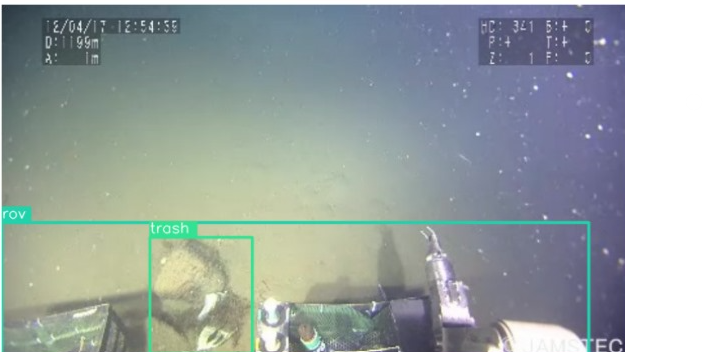
\includegraphics[width=3.5in]{r1.png}
\caption{Detection of Trash and rov.}
\label{fig_1}
\end{figure}

\begin{figure}[!h]
\centering
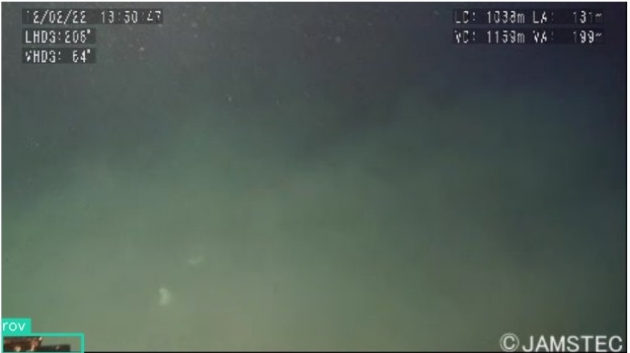
\includegraphics[width=3.5in]{r2.png}
\caption{Detection of rov.}
\label{fig_1}
\end{figure}

\begin{figure}[!h]
\centering
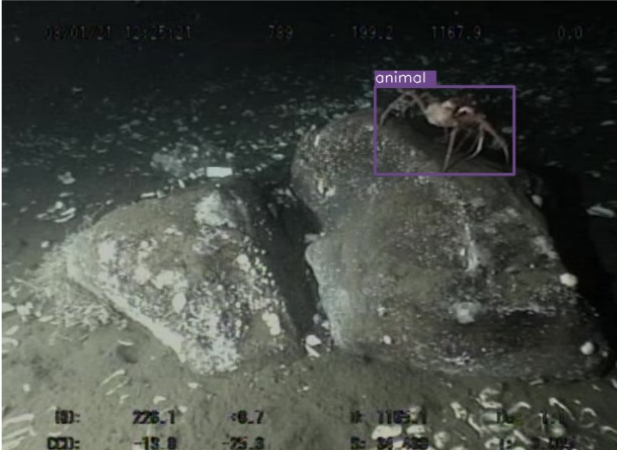
\includegraphics[width=3.5in]{r3.png}
\caption{Detection of Animal.}
\label{fig_1}
\end{figure}

\begin{figure}[!h]
\centering
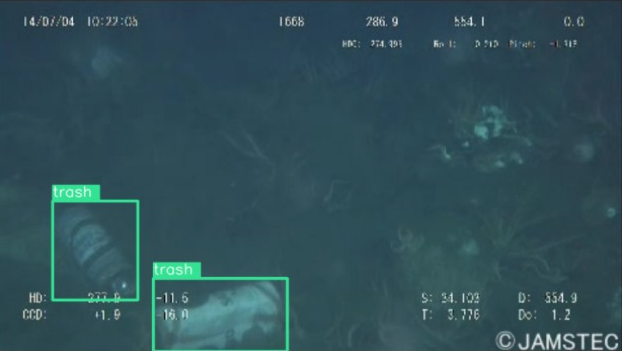
\includegraphics[width=3.5in]{r4.png}
\caption{Detection of Trash.}
\label{fig_1}
\end{figure}






\section{Numerical Results}

Fig.~\ref{fig_2} provides an experimental evaluation of our proposed methodology.

% \begin{figure}[!t]
% \centering
% \includegraphics[width=3.5in]{Fig7.pdf}
% \caption{Simulation results of the proposed approach.}
% \label{fig_2}
% \end{figure}

\section{Conclusion}
Finally, we have suggested a novel strategy for reducing ocean plastic waste that makes use of deep learning and computer vision methods. Our strategy seeks to overcome the drawbacks of conventional marine plastic monitoring techniques and offer an affordable, on-the-spot solution for accurate marine plastic waste identification and quantification.


{\appendices
\section{Key Terms}
\begin{enumerate}
    \item CNN Model: It is one kind of deep learning model that is frequently used for image identification, classification, and segmentation tasks, it stands for convolutional neural network (CNN). Because CNNs can learn complicated patterns straight from raw pixel data and record spatial hierarchies, they are very useful for interpreting visual data. \\
    Training of a CNN involves feeding labeled training data into the network and adjusting its parameters such as filter weights and biases to minimize a loss function and optimize the model's performance. Once the model is trained, the CNN can be used to make predictions on new or unseen data by passing it through the network ,which in turn return us with the output probabilities of each class.\\
    \item AUVs : Unmanned, self-propelled vehicles called autonomous underwater vehicles (AUVs) are made to function underwater without direct human control. These vehicles can move through the water on their own and carry out a variety of functions in underwater settings since they are outfitted with a variety of sensors, navigation systems, and propulsion motors. \\
    The use of this vehicle is mostly related to oceanography, where AUVs are used to collect data from ocean currents, it can read temperature gradients, and observe marine biodiversity, which provide us with valuable insights into oceanographic ecosystems. It is also used in environmental Monitoring where AUVs are deployed to monitor and take reading of environmental parameters like water quality, pollution levels and many more.\\
    \item Object Detection: Finding and detecting things inside an image or video frame is the problem of object detection in computer vision. In contrast to image classification, which assigns a single label to the whole picture, object detection techniques locate and identify many items of interest as well as the bounding boxes that belong to each one. \\
    It invloves processes like Image preprocessing, feature extraction, object classification and post processing. This technology is generally used in autonomous vehicle, in our case the AUVs. It is widely used in medical sector, surveillance and security.
\end{enumerate}

\bibliographystyle{ieeetr}
\bibliography{sc407bib}

\end{document}


